\documentclass[11pt,a4paper]{article}
\usepackage[margin=2.2cm]{geometry}
\usepackage{amsmath,amssymb,bm,braket,booktabs,graphicx,array,enumitem}
\usepackage[dvipsnames]{xcolor}
\usepackage[most]{tcolorbox}
\usepackage{tikz}
\usetikzlibrary{arrows.meta,positioning,calc}
\usepackage{caption}
\usepackage[colorlinks=true,linkcolor=blue!50!black,citecolor=green!40!black,urlcolor=blue!60!black]{hyperref}
\graphicspath{{figs/}{../../Figs.dir/}}
\setlength{\parskip}{0.35em}
\setlist{itemsep=0.15em,topsep=0.3em}

% ---------------------------------------------------------------- source tags
\newcommand{\tagP}[1]{\textcolor{blue!65!black}{\textsf{\small[P:\,#1]}}}
\newcommand{\tagR}[1]{\textcolor{ForestGreen}{\textsf{\small[R:\,#1]}}}
\newcommand{\tagD}{\textcolor{orange!85!black}{\textsf{\small[D]}}}
\newcommand{\tagN}{\textcolor{red!70!black}{\textsf{\small[N]}}}

% ---------------------------------------------------------------- boxes
\newcommand{\plaintags}{\renewcommand{\tagD}{[D]}\renewcommand{\tagN}{[N]}%
  \renewcommand{\tagP}[1]{[P:\,##1]}\renewcommand{\tagR}[1]{[R:\,##1]}}
\newtcolorbox{keybox}[1][]{enhanced,breakable,colback=blue!3,colframe=blue!45!black,
  fonttitle=\bfseries\small\plaintags,title={#1},boxrule=0.6pt,arc=2pt,left=4pt,right=4pt,top=3pt,bottom=3pt}
\newtcolorbox{warnbox}[1][]{enhanced,breakable,colback=red!3,colframe=red!50!black,
  fonttitle=\bfseries\small\plaintags,title={#1},boxrule=0.6pt,arc=2pt,left=4pt,right=4pt,top=3pt,bottom=3pt}
\newtcolorbox{derbox}[1][]{enhanced,breakable,colback=orange!4,colframe=orange!70!black,
  fonttitle=\bfseries\small\plaintags,title={#1},boxrule=0.6pt,arc=2pt,left=4pt,right=4pt,top=3pt,bottom=3pt}
\newtcolorbox{numbox}[1][]{enhanced,breakable,colback=violet!3,colframe=violet!65!black,
  fonttitle=\bfseries\small\plaintags,title={#1},boxrule=0.6pt,arc=2pt,left=4pt,right=4pt,top=3pt,bottom=3pt}

% ---------------------------------------------------------------- physics macros
\newcommand{\bbar}{\bar b b}
\newcommand{\BB}{B\bar B}
\newcommand{\BBst}{B\bar B^*}
\newcommand{\BstBst}{B^*\bar B^*}
\newcommand{\Mth}{M_{\rm th}}
\newcommand{\VQQ}{V^{(\bar bb)}}
\newcommand{\VOME}{V^{\rm (OME)}}
\newcommand{\TOME}{T^{\rm (OME)}}
\newcommand{\bbnP}{[\bar bb]_1(nP)}
\newcommand{\BOchiEFT}{BO$\chi$EFT}
\newcommand{\GeV}{\,\mathrm{GeV}}
\newcommand{\MeV}{\,\mathrm{MeV}}
\newcommand{\D}[2]{\Delta^{(#1)}_{#2}}
\newcommand{\vq}{\bm q}
\newcommand{\vep}{\bm p}
\newcommand{\vn}{\bm n}
\newcommand{\veps}{\bm\epsilon}
\newcommand{\vA}{\bm A}

\title{\textbf{One-meson exchange in the $J^{PC}=2^{++}$ sector}\\[3pt]
\large Partial-wave projection for the $\chi_{b2}(nP)$ extension of Sect.~III\,B and App.~D of\\
``Born--Oppenheimer chiral effective field theory and its application to $X_b$''}
\author{Prepared for Yu Zhang}
\date{21 October 2026}

\begin{document}
\maketitle

\begin{keybox}[How to read this note]
The paper computes the $J^{PC}=1^{++}$ system, i.e.\ the $\chi_{b1}(nP)$ tower coupled to $B^{(*)}\bar B^{*}$. This note does the one-meson-exchange (OME) part of the extension to $J^{PC}=2^{++}$, the $\chi_{b2}(nP)$ tower: which meson-pair channels exist, which TOPT potentials are needed, the $J=2$ projectors, and the partial-wave-projected $6\times6$ OME matrix, in the form of App.~D so that it can be copied into the paper. All conventions (charge-conjugation phase, vertices, TOPT denominators, projection formula, normalisations) are the paper's; nothing is redefined. Every statement carries a source tag:
\begin{itemize}
\item \tagP{Eq.~(80)} --- taken from the paper. Equation, table and section numbers refer to the \emph{current} \texttt{Xb.tex}; \textbf{the \texttt{Xb.pdf} in the project folder is an older build with different numbering.} ``l.\,$n$'' is a line of \texttt{Xb.tex}.
\item \tagR{Ref, location} --- checked in the cited reference (the arXiv \LaTeX{} source was read).
\item \tagD{} --- algebra filled in for this note; it follows from the paper's equations. Re-derive it yourself.
\item \tagN{} --- computed for this note with the scripts in \texttt{code/}. \textbf{Not in the paper.}
\end{itemize}
Units: $\hbar=c=1$, GeV. Energies are measured from the $\BBst$ threshold, $E=M-\Mth$, $\Mth=m_B+m_{B^*}$ \tagP{Eq.~(4)}, also in the $2^{++}$ sector, so that the TOPT denominators of Eq.~(77) can be used unchanged. Potentials are quoted for the exchange of one meson $\phi=\pi,\eta$ and \emph{without} isospin factors, exactly as in Eqs.~(D2)--(D10) \tagP{l.\,1051}.
\end{keybox}

\tableofcontents
\newpage

%=====================================================================
\section{The map: what carries over from $1^{++}$ and what is new}
\label{sec:map}
%=====================================================================

At LO the interaction is $V=\VOME+\sum_{n\le N}\VQQ_n+C(\Lambda,N)$ \tagP{Eq.~(10)}. For the $\chi_{b2}(nP)$ system the same three pieces appear; this note supplies the first one in the $2^{++}$ channel. The paper itself leaves the $\chi_{b0}$ and $\chi_{b2}$ sectors for the future \tagP{l.\,1748}. The extension is technical because every ingredient already exists: the vertices and TOPT denominators are in the paper, and the $J=2$ projectors are in Baru \emph{et al.}\ 2019, App.~B, the reference the paper cites for the projection method \tagP{l.\,1083} \tagR{Baru 2019, App.~B}. What has to be done is to collect the channels, supply the one TOPT potential that does not occur in $1^{++}$, and carry out the angular algebra.

\begin{center}
\small
\begin{tabular}{>{\raggedright\arraybackslash}p{3.7cm}>{\raggedright\arraybackslash}p{4.9cm}>{\raggedright\arraybackslash}p{6.4cm}}
\toprule
ingredient & $1^{++}$ (paper) & $2^{++}$ (this note)\\
\midrule
Lagrangian, vertices & Eqs.~(65)--(70) & unchanged\\
3-body states, $D_\beta$, $\mu_\beta$ & Eqs.~(71), (76), (77), $\beta=1,\dots,4$ & unchanged\\
isospin factors & $3$ ($\pi$), $\frac13$ ($\eta$), Eq.~(82) & unchanged\\
TOPT potentials & $\BBst\!\to\!\BBst$, $\BBst\!\leftrightarrow\!\BstBst$, $\BstBst\!\to\!\BstBst$, Eqs.~(72)--(75) & the same four, plus $\BB\leftrightarrow\BstBst$ (Sect.~\ref{sec:new}); $\BB\to\BB$ and $\BB\leftrightarrow\BBst$ vanish\\
channels & 3, Eq.~(1) & 6, Eq.~\eqref{eq:channels}\\
projectors & Eq.~(D1), one open index & two open indices, Eqs.~\eqref{eq:P1}--\eqref{eq:P6}\\
projection & Eq.~(80), $1/(2J+1)=1/3$ & Eq.~(80), $1/(2J+1)=1/5$\\
angular moments $\D{\beta_1\beta_2}{m}$ & Eq.~(D11): $m\le3$; $(12),(22),(23),(24)$ & $m\le4$; in addition $(33),(44)$\\
result & Eqs.~(D2)--(D10) & Eqs.~\eqref{eq:V11}--\eqref{eq:V55}, time reversal Eq.~\eqref{eq:TR}\\
\bottomrule
\end{tabular}
\end{center}

\begin{figure}[h]
\centering
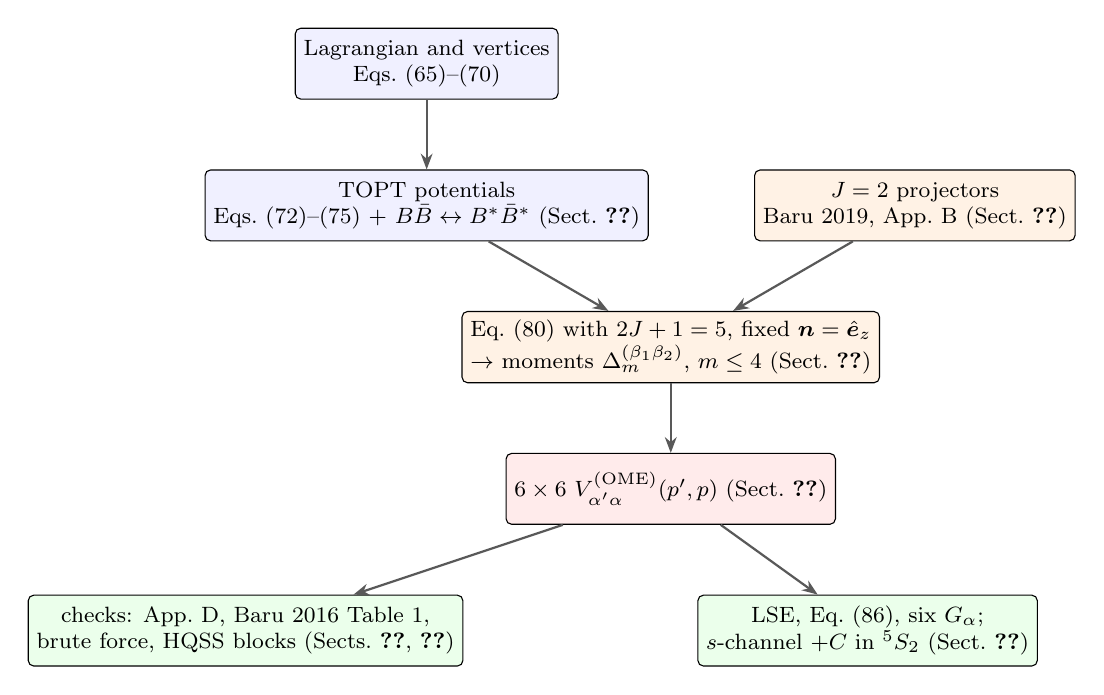
\begin{tikzpicture}[
  box/.style={draw,rounded corners=2pt,align=center,font=\footnotesize,fill=#1,inner sep=3pt,minimum height=0.9cm},
  box/.default=white,
  arr/.style={-{Stealth[length=2mm]},thick,gray!70!black}]
\node[box=blue!6] (lag) at (0,0) {Lagrangian and vertices\\ Eqs.~(65)--(70)};
\node[box=blue!6] (topt) at (0,-1.8) {TOPT potentials\\ Eqs.~(72)--(75) $+$ $\BB\leftrightarrow\BstBst$ (Sect.~\ref{sec:ome})};
\node[box=orange!10] (proj) at (6.2,-1.8) {$J=2$ projectors\\ Baru 2019, App.~B (Sect.~\ref{sec:proj})};
\node[box=orange!10] (pwa) at (3.1,-3.6) {Eq.~(80) with $2J+1=5$, fixed $\vn=\hat{\bm e}_z$\\ $\to$ moments $\D{\beta_1\beta_2}{m}$, $m\le4$ (Sect.~\ref{sec:method})};
\node[box=red!8] (res) at (3.1,-5.4) {$6\times6$ $\VOME_{\alpha'\alpha}(p',p)$ (Sect.~\ref{sec:result})};
\node[box=green!8] (chk) at (-2.3,-7.2) {checks: App.~D, Baru 2016 Table 1,\\ brute force, HQSS blocks (Sects.~\ref{sec:checks}, \ref{sec:hqss})};
\node[box=green!8] (lse) at (5.6,-7.2) {LSE, Eq.~(86), six $G_\alpha$;\\ $s$-channel $+C$ in $^5S_2$ (Sect.~\ref{sec:beyond})};
\draw[arr] (lag) -- (topt);
\draw[arr] (topt) -- (pwa);
\draw[arr] (proj) -- (pwa);
\draw[arr] (pwa) -- (res);
\draw[arr] (res) -- (chk);
\draw[arr] (res) -- (lse);
\end{tikzpicture}
\caption{The steps of this note. Blue: input taken over from the paper; orange: the projection; red: the result; green: what it is checked against and where it goes.}
\label{fig:map}
\end{figure}

Not in this note: the $2^{++}$ versions of the $s$-channel exchange, the contact term and the bare $\chi_{b2}$ tower. Section~\ref{sec:beyond} lists only what must be changed there to use the OME matrix in the LSE.

%=====================================================================
\section{The $2^{++}$ channels}
\label{sec:channels}
%=====================================================================

\subsection{Which meson pairs are $2^{++}$}
\label{sec:channels-list}

For a meson--antimeson pair with orbital angular momentum $L$ and total spin $S$: $P=(-1)^L$, so positive parity needs even $L$; $C=(-1)^{L+S}$ for $\BB$ and $\BstBst$; and $\BBst$ is taken in the $C$-even combination $(\ket{\BBst}-\ket{B^*\bar B})/\sqrt2$ of the paper's phase convention ${\cal C}V{\cal C}^{-1}=-\bar V$ \tagP{l.\,952, footnote~14} (derivation of these rules: \texttt{notes/s\_channel}, Sect.~2.4). Enumerating $J=2$, $P=+$, $C=+$ \tagD:
\begin{center}
\small
\begin{tabular}{lcccl}
\toprule
pair & $S$ & $L$ & $^{2S+1}L_J$ & comment\\
\midrule
$\BB$ & 0 & 2 & $^1D_2$ & $S=0$ forces $L=J=2$; $C=(-1)^2=+$\\
$\BBst$, $C$-even & 1 & 2 & $^3D_2$ & $L=0$ gives $J=1$, $L=4$ gives $J\ge3$\\
$\BBst$, $C$-odd & 1 & --- & --- & $C=-$\\
$\BstBst$ & 0 & 2 & $^1D_2$ & $S=0$ forces $L=2$\\
$\BstBst$ & 1 & --- & --- & $C=(-1)^{L+1}=+$ needs odd $L$, $P=+$ needs even $L$\\
$\BstBst$ & 2 & 0, 2, 4 & $^5S_2$, $^5D_2$, $^5G_2$ & $|L-2|\le2\le L+2$\\
any & $\le2$ & $\ge6$ & --- & $J\ge L-S\ge4$\\
\bottomrule
\end{tabular}
\end{center}
These six channels exhaust the $2^{++}$ pairs; they are the basis of Baru \emph{et al.}\ \tagR{Baru 2016, Eq.~(36); Baru 2017, Eq.~(3.11); Baru 2019, Eq.~(9)}. They are labelled here
\begin{equation}
\alpha=1,\dots,6:\quad
\BstBst(^5S_2),\ \BstBst(^1D_2),\ \BstBst(^5D_2),\ \BstBst(^5G_2),\ \BBst(^3D_2),\ \BB(^1D_2).
\label{eq:channels}
\end{equation}
Two reasons for this order: (i) $\alpha=1$ is the $S$ wave, so the projector $\delta_{\alpha'1}\delta_{\alpha1}$ of the $s$-channel and contact terms in Eq.~(83) keeps its form; (ii) the four $\BstBst$ channels come first, and their $4\times4$ block involves a single TOPT combination, $\D{22}{m}$ (Sect.~\ref{sec:result}). Baru's order, $\BB(^1D_2)$, $\BBst(^3D_2)$, $\BstBst(^5S_2)$, $\BstBst(^1D_2)$, $\BstBst(^5D_2)$, $\BstBst(^5G_2)$, corresponds to $\alpha=6,5,1,2,3,4$. Below, $^1D_2^*$ means $\BstBst(^1D_2)$ and $^1D_2$ means $\BB(^1D_2)$ when the two must be distinguished.

\subsection{Thresholds and two-body propagators}
\label{sec:kin}

With $E=M-\Mth$ and the isospin-limit masses \tagP{Eqs.~(2),(3)} \tagD:
\begin{center}
\small
\begin{tabular}{cllll}
\toprule
$\alpha$ & pair & threshold $-\,\Mth$ & reduced mass & $G_\alpha(k,q)$\\
\midrule
1--4 & $\BstBst$ & $+\Delta m=+46\MeV$ & $m_{B^*}/2=2.663\GeV$ & $\big(q^2/m_{B^*}+\Delta m-E-i\epsilon\big)^{-1}$, the paper's $G_3$\\
5 & $\BBst$ & $0$ & $\mu=2.651\GeV$ & $2\mu/(q^2-k^2-i\epsilon)$, the paper's $G_1$\\
6 & $\BB$ & $-\Delta m=-46\MeV$ & $m_B/2=2.640\GeV$ & $\big(q^2/m_B-\Delta m-E-i\epsilon\big)^{-1}$, new\\
\bottomrule
\end{tabular}
\end{center}
The first two lines are Eq.~(87) \tagP{Eq.~(87)}; the third follows in the same way from $2m_B+q^2/m_B-M$. In contrast to $1^{++}$, the $S$-wave channel has the \emph{highest} threshold: channels 5 and 6 are open for $E>0$ and $E>-\Delta m$. At the $\BstBst$ threshold, $E=\Delta m$, their on-shell momenta are $0.494$ and $0.697\GeV$ \tagN, of the order of the hard scale; a $D$-wave suppression of these transitions cannot be expected. (For the charm analogue Baru \emph{et al.}\ quote $\approx500$ and $700\MeV$ \tagR{Baru 2016, Eqs.~(40),(41)}.) The established $\chi_{b2}(nP)$ lie below all six thresholds: $\chi_{b2}(3P)$ is $10.60\MeV$ above $\chi_{b1}(3P)=10.513\GeV$ \tagP{Table~II, l.\,1739}, i.e.\ at $\approx10.524\GeV$, $34\MeV$ below $2m_B=10.558\GeV$ \tagD.

\subsection{Heavy-quark spin and Born--Oppenheimer content}
\label{sec:hqss-content}

Couple the two heavy spins to $s_{\bar bb}$ and the two light spins to $j_\ell$. In $S$ wave (\texttt{notes/s\_channel}, Sect.~2.5, where the table was checked against Bondar \emph{et al.}\ 2011):
\begin{gather}
\ket{\BB}=\tfrac12\,0_H\!\otimes0_\ell+\tfrac{\sqrt3}{2}(1_H\!\otimes1_\ell)_0,\qquad
\ket{\BstBst}_{S=0}=\tfrac{\sqrt3}{2}\,0_H\!\otimes0_\ell-\tfrac12(1_H\!\otimes1_\ell)_0,\notag\\
\ket{\BBst;+}=(1_H\!\otimes1_\ell)_1,\qquad
\ket{\BstBst}_{S=2}=(1_H\!\otimes1_\ell)_2 .
\label{eq:hl}
\end{gather}
With even $L$, $C=C_\ell C_H$ and $P=+$, so a $2^{++}$ state needs $(s_{\bar bb},j_\ell)=(0,0)$ or $(1,1)$ \tagP{Eqs.~(15),(16)} \tagD. Coupling $\bm J_\ell=\bm L+\bm j_\ell$ first \tagP{l.\,493--495}:
\begin{center}
\small
\begin{tabular}{llll}
\toprule
$(s_{\bar bb},j_\ell)$ & $J_\ell$ & $L$ & in $1^{++}$?\\
\midrule
$(0,0)$ & 2 & 2 & no\\
$(1,1)$ & 1 & 0, 2 & yes (the $^3S_1$--$(2,1)1$ pair of Eq.~(20))\\
$(1,1)$ & 2 & 2 & yes ($(2,1)2$ of Eq.~(20))\\
$(1,1)$ & 3 & 2, 4 & no\\
\bottomrule
\end{tabular}
\end{center}
Six states, as many as channels \tagD. The $J_\ell=1$ and $J_\ell=2$ states are common to $1^{++}$ and $2^{++}$; heavy-quark spin symmetry (HQSS) therefore relates the two OME matrices (Sect.~\ref{sec:hqss}). New in $2^{++}$ are the light-spin singlet and $J_\ell=3$. In Born--Oppenheimer (BO) language the light singlet is $\Sigma_u^-$, which cannot contribute to $1^{++}$ \tagP{l.\,505} but does contribute to $2^{++}$ with $L=2$, $s_{\bar bb}=0$; the count is $\Sigma_u^-$ (1) $+$ $\Sigma_g^{+\prime}$ with $J_\ell=1,3$ (2) $+$ $\Pi_g$ with $J_\ell=1,2,3$ (3) $=6$. As in $1^{++}$, there is no $\lambda_\ell=0$ state with $J_\ell=L=2$ \tagP{l.\,497--504} \tagD.

%=====================================================================
\section{The OME potentials needed in $2^{++}$}
\label{sec:ome}
%=====================================================================

\subsection{Taken over unchanged}

The potentials between $C$-even $\BBst$ and $\BstBst$ states are those of Eqs.~(72)--(75) \tagP{Eqs.~(72)--(75)}. They are operators in polarisation space, so they do not know about $J$; only the projection does. The conventions of l.\,1052 carry over: in Eqs.~(73) and (74) the two terms are the $\BBst$ and $B^*\bar B$ components of the $C$-even state, and $\vA_a=\frac{i}{\sqrt2}(\veps_a\times\veps_a^{\prime*})$ sits on line $a=1$ ($B^*$) or $a=2$ ($\bar B^*$) \tagP{l.\,1052}. The TOPT denominators $D_\beta=1/\{2E_\phi(q)[E_\phi(q)+\mu_\beta]\}$ and the $\mu_\beta$ are Eqs.~(76), (77) \tagP{Eqs.~(76),(77)}.

\subsection{Vanishing transitions}

There is no $BB\phi$ vertex: $0^-\to0^-0^-$ violates parity, and Eq.~(68) has no $P^\dagger P$ or $\bar P^\dagger\bar P$ term \tagP{Eq.~(68)}. One-meson exchange needs one vertex on each meson line, so
\begin{equation}
V_{\BB\to\BB}=V_{\BB\to\BBst}=V_{\BBst\to\BB}=0
\end{equation}
identically, for any masses \tagD. Hence $V_{56}=V_{65}=V_{66}=0$.

\subsection{The new transition $\BB\leftrightarrow\BstBst$}
\label{sec:new}

Both lines change $B\to B^*$, through the vertex of Eq.~(69). The result, in the paper's conventions \tagD:
\begin{keybox}[New TOPT potential (not in the paper)]
\begin{align}
\VOME_{\BB\to\BstBst}(\bm p',\bm p;m_\phi)&=\frac{g_b^2}{4F_\pi^2}\,(\veps_1^{\prime*}\cdot\vq)(\veps_2^{\prime*}\cdot\vq)\,\big[2D_3(\bm p',\bm p;m_\phi)\big],\label{eq:VPPVV}\\
\VOME_{\BstBst\to\BB}(\bm p',\bm p;m_\phi)&=\frac{g_b^2}{4F_\pi^2}\,(\veps_1\cdot\vq)(\veps_2\cdot\vq)\,\big[2D_4(\bm p',\bm p;m_\phi)\big],\label{eq:VVVPP}
\end{align}
with $\vq=\vep-\vep'$, $\veps_{1}$ ($\veps_2$) the polarisation of the $B^*$ ($\bar B^*$), and $D_{3,4}$ of Eqs.~(76),(77). The isospin factors are those of Eq.~(82).
\end{keybox}

\begin{derbox}[Derivation \tagD]
\textbf{Trace form of the vertices.} Write a meson as a $2\times2$ matrix in heavy$\otimes$light spin, as in $H=P+\bm V\cdot\bm\sigma$ \tagP{l.\,953--958}: $M_B=\frac{1}{\sqrt2}$, $M_{B^*}(\veps)=\frac{1}{\sqrt2}\veps\cdot\bm\sigma$ (so ${\rm Tr}\,M^\dagger M=1$), and the same for antimesons. With $\bm u=-\bm\nabla\Phi/F_\pi$, Eq.~(65) gives $\frac{g_b}{4F_\pi}{\rm Tr}(H^\dagger H\sigma_k)\partial_k\Phi-\frac{g_b}{4F_\pi}{\rm Tr}(\sigma_k\bar H\bar H^\dagger)\partial_k\Phi$. Evaluating the traces reproduces every term of Eq.~(68). A meson line therefore contributes $t_1={\rm Tr}[M_1^{\prime\dagger}M_1\,\bm\sigma\cdot\vq]$ and an antimeson line $t_2={\rm Tr}[\bm\sigma\cdot\vq\,\bar M_2\bar M_2^{\prime\dagger}]$. The overall minus sign of the antimeson term, the factors $i$ from $\partial_k\Phi$, the TOPT sign and the isospin structure are the same for every transition. They combine into one constant $K$:
\[
V_{fi}=K\,t_1\,t_2\,\textstyle\sum_{\rm orderings}D_\beta .
\]
The line factors are
\begin{center}
\small
\begin{tabular}{lcccc}
\toprule
& $B\to B$ & $B\to B^*$ & $B^*\to B$ & $B^*\to B^*$\\
\midrule
meson, $t_1$ & 0 & $\veps^{\prime*}\cdot\vq$ & $\veps\cdot\vq$ & $i(\veps^{\prime*}\times\veps)\cdot\vq=-\sqrt2\,\vA\cdot\vq$\\
antimeson, $t_2$ & 0 & $\veps^{\prime*}\cdot\vq$ & $\veps\cdot\vq$ & $i(\veps\times\veps^{\prime*})\cdot\vq=+\sqrt2\,\vA\cdot\vq$\\
\bottomrule
\end{tabular}
\end{center}
\textbf{Calibration on the paper.} (a) $\BstBst\to\BstBst$: $t_1t_2=-2(\vA_1\cdot\vq)(\vA_2\cdot\vq)$, with both orderings through $\BstBst\phi$; Eq.~(75) fixes $K=g_b^2/(4F_\pi^2)$. (b) $\BBst\to\BBst$ with $\ket{+}=(\ket{\BBst}-\ket{B^*\bar B})/\sqrt2$: the direct terms need $B\to B$ or $\bar B\to\bar B$ on one line and vanish, leaving $-\frac12\big[\braket{\BBst|V|B^*\bar B}+\braket{B^*\bar B|V|\BBst}\big]=-K(\veps\cdot\vq)(\veps^{\prime*}\cdot\vq)[D_1+D_2]$. That is Eq.~(72). (c) $\BBst\to\BstBst$: $\frac{1}{\sqrt2}\big[(\veps_1^{\prime*}\cdot\vq)(\sqrt2\vA_2\cdot\vq)-(-\sqrt2\vA_1\cdot\vq)(\veps_2^{\prime*}\cdot\vq)\big]=(\vA_1\cdot\vq)(\veps_2^{\prime*}\cdot\vq)+(\vA_2\cdot\vq)(\veps_1^{\prime*}\cdot\vq)$, which is Eq.~(73). Eq.~(74) follows the same way. No free constant or sign is left.

\textbf{The new element.} For $\BB\to\BstBst$, $t_1t_2=(\veps_1^{\prime*}\cdot\vq)(\veps_2^{\prime*}\cdot\vq)$. The two time orderings have the intermediate states $B^*(\bm p')\bar B(-\bm p)\phi$ and $B(\bm p)\bar B^*(-\bm p')\phi$. Both contain a pseudoscalar with the incoming momentum $p$ and a vector with the outgoing momentum $p'$, which is $\mu_3=E_B(p)+E_{B^*}(p')-M$ of Eq.~(77). Hence $[D_3+D_3]$ and Eq.~\eqref{eq:VPPVV}. Hermitian conjugation, together with $D_3(\bm p,\bm p')=D_4(\bm p',\bm p)$ \tagP{l.\,2137}, gives Eq.~\eqref{eq:VVVPP}.
\end{derbox}

\paragraph{Comparison with the literature.} Baru \emph{et al.}\ have the same structure, $(\veps_1^{\prime*}\cdot\vq)(\veps_2^{\prime*}\cdot\vq)\,2/D_{BB^*\pi}$, with $D_{BB^*\pi}$ the $\mu_3$ denominator \tagR{Baru 2017, Eqs.~(3.5),(3.7); Baru 2019, Eqs.~(43),(47)}. Their normalisation differs: they absorb the integration weight into $V$, use the isovector factor, and in 2017 write $\vq=\vep+\vep'$. Their relative sign between $V_{\BB\to\BstBst}$ and $V_{\BstBst\to\BstBst}$ is opposite to ours, because they use ${\cal C}\hat M=\bar M$ for all mesons \tagR{Baru 2017, Eq.~(2.2); Baru 2019, Eqs.~(10),(11)}, while the paper uses ${\cal C}V{\cal C}^{-1}=-\bar V$ \tagP{l.\,952}. The two conventions differ by the phase of every $\bar B^*$ state. That flips $V_{\BB\to\BstBst}$ and leaves Eqs.~(72)--(75) unchanged; it is equivalent to flipping the sign of the $\BB$ basis state, so no observable changes \tagD.

\subsection{Summary}
\label{sec:ome-summary}

\begin{center}
\small
\begin{tabular}{llcl}
\toprule
out $\leftarrow$ in & spin structure & prefactor & $[D_{\beta_1}+D_{\beta_2}]$\\
\midrule
$\BBst\leftarrow\BBst$ & $(\veps\cdot\vq)(\veps^{\prime*}\cdot\vq)$ & $-g_b^2/4F_\pi^2$ & $D_1+D_2$ \quad Eq.~(72)\\
$\BstBst\leftarrow\BBst$ & $(\vA_1\cdot\vq)(\veps_2^{\prime*}\cdot\vq)+(\vA_2\cdot\vq)(\veps_1^{\prime*}\cdot\vq)$ & $+g_b^2/4F_\pi^2$ & $D_3+D_2$ \quad Eq.~(73)\\
$\BBst\leftarrow\BstBst$ & $(\vA_1\cdot\vq)(\veps_2\cdot\vq)+(\vA_2\cdot\vq)(\veps_1\cdot\vq)$ & $+g_b^2/4F_\pi^2$ & $D_4+D_2$ \quad Eq.~(74)\\
$\BstBst\leftarrow\BstBst$ & $(\vA_1\cdot\vq)(\vA_2\cdot\vq)$ & $-g_b^2/2F_\pi^2$ & $2D_2$ \quad Eq.~(75)\\
$\BstBst\leftarrow\BB$ & $(\veps_1^{\prime*}\cdot\vq)(\veps_2^{\prime*}\cdot\vq)$ & $+g_b^2/4F_\pi^2$ & $2D_3$ \quad Eq.~\eqref{eq:VPPVV}\\
$\BB\leftarrow\BstBst$ & $(\veps_1\cdot\vq)(\veps_2\cdot\vq)$ & $+g_b^2/4F_\pi^2$ & $2D_4$ \quad Eq.~\eqref{eq:VVVPP}\\
$\BB\leftarrow\BB$, $\BB\leftrightarrow\BBst$ & --- & 0 & ---\\
\bottomrule
\end{tabular}
\end{center}

%=====================================================================
\section{Projectors for $J=2$}
\label{sec:proj}
%=====================================================================

Baru \emph{et al.}\ 2019 list a complete set of projectors for $0^{++}$, $1^{+-}$, $1^{++}$ and $2^{++}$ \tagR{Baru 2019, App.~B, Eqs.~(B1)--(B19)}. Their $1^{++}$ projectors (B5), (B6), (B12) coincide with the paper's Eq.~(D1), signs included \tagR{Baru 2019, Eqs.~(B5),(B6),(B12)} \tagP{Eq.~(D1)}. Their $2^{++}$ projectors therefore extend the paper's phase conventions, and are used here unchanged. With $\vn=\hat{\bm p}$,
\begin{align}
P_{ij}\big(\BstBst(^5S_2)\big)&=\tfrac12\,S_{ij},\label{eq:P1}\\
P_{ij}\big(\BstBst(^1D_2)\big)&=-\sqrt{\tfrac52}\,(\veps_1\cdot\veps_2)\,v_{ij},\\
P_{ij}\big(\BstBst(^5D_2)\big)&=-\sqrt{\tfrac{45}{56}}\Big(S_{ik}v_{kj}+S_{jk}v_{ki}-\tfrac23\delta_{ij}S_{kl}v_{kl}\Big),\\
P_{ij}\big(\BstBst(^5G_2)\big)&=\sqrt{\tfrac{175}{32}}\,S_{kl}\,v_{ijkl},\\
P_{ij}\big(\BBst(^3D_2)\big)&=-\tfrac{\sqrt5}{2}\,\epsilon_k\big(i\varepsilon_{ikl}v_{lj}+i\varepsilon_{jkl}v_{li}\big),\\
P_{ij}\big(\BB(^1D_2)\big)&=-\sqrt{\tfrac{15}{2}}\,v_{ij},\label{eq:P6}
\end{align}
\tagR{Baru 2019, Eqs.~(B10),(B11),(B13),(B14),(B7),(B4)}, where \tagR{Baru 2019, Eqs.~(B15)--(B18)}
\begin{gather}
v_{ij}=n_in_j-\tfrac13\delta_{ij},\qquad
S_{ij}=\epsilon_{1i}\epsilon_{2j}+\epsilon_{1j}\epsilon_{2i}-\tfrac23\delta_{ij}\,\veps_1\cdot\veps_2,\notag\\
v_{ijkl}=n_in_jn_kn_l-\tfrac17\big(n_in_j\delta_{kl}+n_in_k\delta_{jl}+n_in_l\delta_{jk}+n_jn_k\delta_{il}+n_jn_l\delta_{ik}+n_kn_l\delta_{ij}\big)\notag\\
\hspace*{5cm}+\tfrac1{35}\big(\delta_{ij}\delta_{kl}+\delta_{ik}\delta_{jl}+\delta_{il}\delta_{jk}\big).
\end{gather}
How to read them (cf.\ \texttt{notes/s\_channel}, Sect.~2.9):
\begin{itemize}
\item the open pair $ij$ is symmetric and traceless: five components, the polarisation tensor of the $J=2$ state. This is why $J=2$ projectors have two open indices;
\item $v_{ij}$ and $v_{ijkl}$ are the rank-2 and rank-4 harmonic tensors of $\vn$, i.e.\ $L=2$ and $L=4$; no $\vn$ means $L=0$;
\item $\veps_1\cdot\veps_2$ is the $S=0$ state of two vector mesons, $S_{ij}$ the $S=2$ state, and a single $\veps$ is $S=1$;
\item $i\varepsilon_{ikl}\epsilon_kv_{lj}$ couples $S=1$ and $L=2$ to a rank-2 tensor, symmetrised in $ij$ and automatically traceless because $\varepsilon_{ikl}v_{li}=0$; $S_{ik}v_{kj}+\dots$ is the $J=2$ part of $S=2\otimes L=2$; $S_{kl}v_{ijkl}$ contracts two of the four $L=4$ indices with $S=2$.
\end{itemize}
Each tensor has definite $L$, $S$ and $J=2$. Since each $(L,S,J)$ occurs once, the projectors are the $\ket{(LS)J}$ states up to phases. With $1/(2J+1)=1/5$ in Eq.~(81), all six are normalised, and the four $\BstBst$ projectors are mutually orthogonal \tagN. The phases matter only for comparisons with standard recoupling tables; see the box at the end of Sect.~\ref{sec:hqss}.

%=====================================================================
\section{Partial-wave projection}
\label{sec:method}
%=====================================================================

\subsection{Reduction to one angle}

The projection is Eq.~(80) with $J=2$ \tagP{Eqs.~(80),(81)}:
\begin{equation}
\VOME_{\alpha'\alpha}(p',p;m_\phi)=\frac15\int\frac{d\Omega_{\vn'}}{4\pi}\frac{d\Omega_{\vn}}{4\pi}\,{\rm Tr}\Big[P^\dagger(\alpha';\vn')\,\VOME(\bm p',\bm p;m_\phi)\,P(\alpha;\vn)\Big],
\end{equation}
the trace running over the open indices $ij$ and all polarisations, with $\veps$ for incoming and $\veps^{\prime*}$ for outgoing mesons contracted through $\sum_\lambda\epsilon_a(\lambda)\epsilon^*_b(\lambda)=\delta_{ab}$. Steps \tagD:
\begin{enumerate}
\item The trace is a rotational scalar, so the double average equals the average over $\vn'$ at fixed $\vn=\hat{\bm e}_z$.
\item Write $\vn'=(\sin\theta'\cos\varphi',\sin\theta'\sin\varphi',x)$ and $\vq=p\hat{\bm e}_z-p'\vn'$. The $D_\beta$ depend on $\vq$ only through $q^2=p^2+p^{\prime2}-2pp'x$ \tagP{Eqs.~(D12),(D13)}, so the $\varphi'$ average acts on the polynomial numerator alone. After it, $\sin^2\theta'=1-x^2$ leaves a polynomial $T_{\alpha'\alpha}(x;p',p)$.
\item Hence $\VOME_{\alpha'\alpha}=\frac{c}{5}\cdot\frac12\int_{-1}^1dx\,T_{\alpha'\alpha}(x)\,[D_{\beta_1}+D_{\beta_2}]$, with $c$ the prefactor of the table in Sect.~\ref{sec:ome-summary}. In terms of the moments of Eq.~(D11),
\begin{equation}
\D{\beta_1\beta_2}{m}(p',p;m_\phi)=\int_{-1}^1x^m\,dx\,\big[D_{\beta_1}(p',p,x;m_\phi)+D_{\beta_2}(p',p,x;m_\phi)\big],
\label{eq:Delta}
\end{equation}
the coefficient of $\D{\beta_1\beta_2}{m}$ is $c\,T^{(m)}_{\alpha'\alpha}/10$, with $T^{(m)}$ the coefficient of $x^m$.
\end{enumerate}
Two new combinations appear, $\D{33}{m}$ and $\D{44}{m}$, with $\D{44}{m}(p',p)=\D{33}{m}(p,p')$. Moments up to $m=4$ occur \tagN. Naively the $^5G_2\to{}^5G_2$ element could contain $x^5$ ($P_4(x)$ times the $x$ in $q^2$), but that term cancels, as $x^3$ cancels in the $1^{++}$ state $(2,1)J_\ell{=}1$ (Sect.~\ref{sec:hqss}) \tagN. The analytic evaluation of App.~D, the change of variables $x\to E_\phi$ that leads to Eq.~(D15), works for any $m$ \tagP{Eqs.~(D15)--(D17)}. At ${\cal B}=2pp'=0$ the $D_\beta$ do not depend on $x$, so Eq.~(D17) generalises to $\D{\beta_1\beta_2}{m}\big|_{{\cal B}=0}=\D{\beta_1\beta_2}{0}\big|_{{\cal B}=0}/(m+1)$ for even $m$ and $0$ for odd $m$ \tagD.

\subsection{A worked example: $^5S_2\to{}^5S_2$}

\begin{derbox}[$V_{11}$ with spin operators \tagD]
Write $(S_k)_{ba}=-i\varepsilon_{kba}$ for the spin-1 matrices. Then $\vA\cdot\vq=\frac{1}{\sqrt2}\braket{\veps'|\bm S\cdot\vq|\veps}$ and
\begin{gather*}
(\vA_1\cdot\vq)(\vA_2\cdot\vq)=\tfrac12\braket{\veps_1'\veps_2'|(\bm S_1\cdot\vq)(\bm S_2\cdot\vq)|\veps_1\veps_2},\\
(\bm S_1\cdot\vq)(\bm S_2\cdot\vq)=\tfrac13q^2\,\bm S_1\cdot\bm S_2+\big(q_iq_j-\tfrac13\delta_{ij}q^2\big)S_{1i}S_{2j}.
\end{gather*}
Both $^5S_2$ projectors are $\vn$ independent, and $\frac15{\rm Tr}[P^\dagger(\dots)P]$ is the average over the five $S=2$ states. The rank-2 spin tensor has zero trace over a complete multiplet (Wigner--Eckart). On $S=2$, $\bm S_1\cdot\bm S_2=\frac12[S(S+1)-2-2]=1$. So $\frac15{\rm Tr}=\frac12\cdot\frac13q^2$, and with the prefactor of Eq.~(75),
\[
V_{11}=-\frac{g_b^2}{2F_\pi^2}\cdot\frac16\cdot\frac12\!\int_{-1}^1\!dx\,q^2\,[2D_2]
=\frac{g_b^2}{24F_\pi^2}\Big[2pp'\D{22}{1}-(p^2+p^{\prime2})\D{22}{0}\Big].
\]
For $1^{++}$, $(\veps\cdot\vq)(\veps^{\prime*}\cdot\vq)$ averaged over the three $^3S_1$ states gives $\frac13q^2$, and Eq.~(72) leads to Eq.~(D2): the same expression with $\D{12}{m}$. The $S$-wave OME of the $2^{++}$ spin partner differs from that of the $X_b$ channel \emph{only} through the TOPT denominators: $2D_2$ (intermediate $\BstBst\phi$ in both orderings) instead of $D_1+D_2$.
\end{derbox}

\subsection{Validation on $1^{++}$}

The same code applied to the three $1^{++}$ channels with the projectors of Eq.~(D1) reproduces all nine elements of Eqs.~(D2)--(D10) exactly, including the assignment of $\D{12}{m}$, $\D{24}{m}$, $\D{23}{m}$, $\D{22}{m}$ and the time-reversed elements (D5), (D8), (D9) \tagN.

%=====================================================================
\section{Result: the projected $2^{++}$ OME}
\label{sec:result}
%=====================================================================

\begin{keybox}[The $2^{++}$ OME matrix (the analogue of Eqs.~(D2)--(D10)) \tagN]
Channels as in Eq.~\eqref{eq:channels}: $1={}^5S_2$, $2={}^1D_2^*$, $3={}^5D_2$, $4={}^5G_2$ (all $\BstBst$), $5=\BBst(^3D_2)$, $6=\BB(^1D_2)$. All $\D{\beta_1\beta_2}{m}\equiv\D{\beta_1\beta_2}{m}(p',p;m_\phi)$, with $p'$ ($p$) the outgoing (incoming) momentum.
{\small
\begin{align}
V_{11}&=\frac{g_b^2}{24F_\pi^2}\Big[2pp'\D{22}{1}-(p^2+p^{\prime2})\D{22}{0}\Big],\label{eq:V11}\\[1mm]
V_{12}&=\frac{g_b^2}{24\sqrt{10}\,F_\pi^2}\Big[3p^{\prime2}\D{22}{2}-4pp'\D{22}{1}+(2p^2-p^{\prime2})\D{22}{0}\Big],\\[1mm]
V_{13}&=-\frac{\sqrt7\,g_b^2}{24\sqrt{10}\,F_\pi^2}\Big[3p^{\prime2}\D{22}{2}-4pp'\D{22}{1}+(2p^2-p^{\prime2})\D{22}{0}\Big],\\[1mm]
V_{14}&=0,\\[1mm]
V_{15}&=-\frac{g_b^2}{8\sqrt{10}\,F_\pi^2}\Big[3p^{\prime2}\D{23}{2}-4pp'\D{23}{1}+(2p^2-p^{\prime2})\D{23}{0}\Big],\\[1mm]
V_{16}&=-\frac{\sqrt3\,g_b^2}{24\sqrt{10}\,F_\pi^2}\Big[3p^{\prime2}\D{33}{2}-4pp'\D{33}{1}+(2p^2-p^{\prime2})\D{33}{0}\Big],\\[1mm]
V_{22}&=-\frac{g_b^2}{24F_\pi^2}\Big[6pp'\D{22}{3}-3(p^2+p^{\prime2})\D{22}{2}-2pp'\D{22}{1}+(p^2+p^{\prime2})\D{22}{0}\Big],\\[1mm]
V_{23}&=\frac{g_b^2}{24\sqrt7\,F_\pi^2}\Big[3pp'\D{22}{3}-3(p^2+p^{\prime2})\D{22}{2}+pp'\D{22}{1}+(p^2+p^{\prime2})\D{22}{0}\Big],\\[1mm]
V_{24}&=\frac{g_b^2}{32\sqrt{35}\,F_\pi^2}\Big[35p^{\prime2}\D{22}{4}-40pp'\D{22}{3}+6(2p^2-5p^{\prime2})\D{22}{2}+24pp'\D{22}{1}-(4p^2-3p^{\prime2})\D{22}{0}\Big],\\[1mm]
V_{25}&=0,\\[1mm]
V_{26}&=-\frac{\sqrt3\,g_b^2}{48F_\pi^2}\Big[6pp'\D{33}{3}-3(p^2+p^{\prime2})\D{33}{2}-2pp'\D{33}{1}+(p^2+p^{\prime2})\D{33}{0}\Big],\\[1mm]
V_{33}&=\frac{g_b^2}{336F_\pi^2}\Big[51pp'\D{22}{3}-30(p^2+p^{\prime2})\D{22}{2}-11pp'\D{22}{1}+10(p^2+p^{\prime2})\D{22}{0}\Big],\\[1mm]
V_{34}&=-\frac{g_b^2}{112\sqrt5\,F_\pi^2}\Big[35p^{\prime2}\D{22}{4}-40pp'\D{22}{3}+6(2p^2-5p^{\prime2})\D{22}{2}+24pp'\D{22}{1}-(4p^2-3p^{\prime2})\D{22}{0}\Big],\\[1mm]
V_{35}&=-\frac{g_b^2}{16\sqrt7\,F_\pi^2}\Big[3pp'\D{23}{3}-3(p^2+p^{\prime2})\D{23}{2}+pp'\D{23}{1}+(p^2+p^{\prime2})\D{23}{0}\Big],\\[1mm]
V_{36}&=-\frac{g_b^2}{8\sqrt{21}\,F_\pi^2}\Big[3pp'\D{33}{3}-3(p^2+p^{\prime2})\D{33}{2}+pp'\D{33}{1}+(p^2+p^{\prime2})\D{33}{0}\Big],\\[1mm]
V_{44}&=\frac{g_b^2}{448F_\pi^2}\Big[35(p^2+p^{\prime2})\D{22}{4}-40pp'\D{22}{3}-30(p^2+p^{\prime2})\D{22}{2}+24pp'\D{22}{1}+3(p^2+p^{\prime2})\D{22}{0}\Big],\\[1mm]
V_{45}&=\frac{g_b^2}{16\sqrt{35}\,F_\pi^2}\Big[35p^2\D{23}{4}-40pp'\D{23}{3}-6(5p^2-2p^{\prime2})\D{23}{2}+24pp'\D{23}{1}+(3p^2-4p^{\prime2})\D{23}{0}\Big],\\[1mm]
V_{46}&=-\frac{\sqrt3\,g_b^2}{32\sqrt{35}\,F_\pi^2}\Big[35p^2\D{33}{4}-40pp'\D{33}{3}-6(5p^2-2p^{\prime2})\D{33}{2}+24pp'\D{33}{1}+(3p^2-4p^{\prime2})\D{33}{0}\Big],\\[1mm]
V_{55}&=\frac{g_b^2}{16F_\pi^2}\,pp'\Big[\D{12}{3}-\D{12}{1}\Big],\label{eq:V55}\\[1mm]
V_{56}&=V_{66}=0.\notag
\end{align}}
The remaining elements follow from time reversal \tagN,
\begin{gather}
V_{\alpha\alpha'}(p',p;m_\phi)=V_{\alpha'\alpha}(p,p';m_\phi),\notag\\
\text{with}\quad \D{23}{m}(p,p')=\D{24}{m}(p',p),\qquad \D{33}{m}(p,p')=\D{44}{m}(p',p),
\label{eq:TR}
\end{gather}
as for $V_{31}$ and $V_{32}$ in App.~D \tagP{l.\,2137}. For example, $V_{51}=-\frac{g_b^2}{8\sqrt{10}F_\pi^2}\big[3p^2\D{24}{2}-4pp'\D{24}{1}+(2p^{\prime2}-p^2)\D{24}{0}\big]$. The full isoscalar matrix is Eq.~(82) unchanged: $\VOME_{\alpha'\alpha}=3\VOME_{\alpha'\alpha}(m_\pi)+\frac13\VOME_{\alpha'\alpha}(m_\eta)$.
\end{keybox}

\paragraph{Which TOPT combination enters where.} This follows from the table of Sect.~\ref{sec:ome-summary} \tagD:
\begin{center}
\small
\begin{tabular}{c|cccc|c|c}
out $\backslash$ in & 1 & 2 & 3 & 4 & 5 & 6\\
\hline
1--4 ($\BstBst$) & $(22)$ & $(22)$ & $(22)$ & $(22)$ & $(23)$ & $(33)$\\
5 ($\BBst$) & $(24)$ & $(24)$ & $(24)$ & $(24)$ & $(12)$ & ---\\
6 ($\BB$) & $(44)$ & $(44)$ & $(44)$ & $(44)$ & --- & ---\\
\end{tabular}
\end{center}
Besides the zeros forced by the missing $BB\phi$ vertex, two elements vanish identically for any masses \tagN:
\begin{itemize}
\item $V_{14}=V_{41}=0$. Both channels are $\BstBst$ and use only $2D_2$; the operator conserves $J_\ell$ (Sect.~\ref{sec:hqss}); $^5S_2$ is pure $J_\ell=1$ and $^5G_2$ pure $J_\ell=3$. The $G$ wave couples to the $S$ wave only through the $D$-wave channels.
\item $V_{25}=V_{52}=0$. The spin part of every OME is a sum of rank-0 and rank-2 tensors in spin space. Rank 0 conserves $S$, and rank 2 cannot connect $S=1$ to $S=0$ (no triangle $1,2,0$); cf.\ $\sum_b\varepsilon_{kab}q_kq_b=0$ in Eq.~(73) contracted with $\delta_{b_1b_2}$.
\end{itemize}
The $S$-wave row has the $D$-wave bracket of Eqs.~(D3),(D4) in every entry, and $V_{23}$, $V_{35}$, $V_{36}$ have the bracket of Eq.~(D7). $V_{55}$ equals Eq.~(D10) with $\D{22}{}\to\D{12}{}$ \tagN.

\paragraph{Where it enters.} The total $2^{++}$ potential has the form of Eq.~(83) with $\alpha=1$ the $^5S_2$ channel, and the LSE is Eq.~(86) with the six propagators of Sect.~\ref{sec:kin} \tagP{Eqs.~(83),(86)} \tagD.

%=====================================================================
\section{Checks}
\label{sec:checks}
%=====================================================================

\begin{numbox}[What was checked, and how \tagN]
\begin{enumerate}
\item \textbf{The method on $1^{++}$.} The code that produced Sect.~\ref{sec:result}, run with Eq.~(D1), reproduces Eqs.~(D2)--(D10) symbolically, element by element, including the $\D{\beta_1\beta_2}{}$ labels (\texttt{pwa.py}).
\item \textbf{Projectors.} $\frac15\langle{\rm Tr}\,P(\alpha)P^\dagger(\beta)\rangle_\Omega=\delta_{\alpha\beta}$ exactly for the four $\BstBst$ projectors, and $=1$ for $^3D_2$ and $\BB(^1D_2)$; the same holds for Eq.~(D1) with $\frac13$ (\texttt{checks.py}).
\item \textbf{Time reversal}, Eq.~\eqref{eq:TR}, symbolically for all 36 elements (\texttt{pwa.py}).
\item \textbf{Brute force.} For physical masses, $g_b=0.56$, $F_\pi=92.2\MeV$, $E=-120\MeV$ (below all thresholds), $(p,p')=(0.31,0.57)$ and $(0.83,0.22)\GeV$, and both $m_\pi$ and $m_\eta$, Eq.~(80) is evaluated by direct quadrature over \emph{both} spheres with the full TOPT denominators at every $\vq$, without the reduction of Sect.~\ref{sec:method}. The maximum deviation from Sect.~\ref{sec:result}, relative to the largest element, is $2\times10^{-12}$ for $2^{++}$ and $7\times10^{-13}$ for $1^{++}$ (on a $30\times36$ grid per sphere; $1.5\times10^{-8}$ on $20\times24$, so the agreement is set by quadrature) (\texttt{numcheck.py}).
\item \textbf{One-loop leading divergences.} In the static HQSS limit Baru \emph{et al.}\ split the leading UV divergence of the iterated OPE in $^3S_1\to{}^3S_1$ ($1^{++}$) and $^5S_2\to{}^5S_2$ ($2^{++}$) into intermediate partial waves \tagR{Baru 2016, Table~1}. The weight of channel $\alpha$ is $|V_{\alpha S}(l,0)|^2/\sum_\beta|V_{\beta S}(l,0)|^2$. From Eqs.~(D2)--(D4) and Sect.~\ref{sec:result} (\texttt{checks.py}):
\begin{center}
\small
\begin{tabular}{lcccccc}
\toprule
$1^{++}$ & $^3S_1$ & $^3D_1$ & $^5D_1$ &&&\\
here $=$ Baru & $1/9$ & $2/9$ & $2/3$ &&&\\
\midrule
$2^{++}$ & $\BB(^1D_2)$ & $\BBst(^3D_2)$ & $^5S_2$ & $^1D_2^*$ & $^5D_2$ & $^5G_2$\\
here $=$ Baru & $2/15$ & $2/5$ & $1/9$ & $2/45$ & $14/45$ & $0$\\
\bottomrule
\end{tabular}
\end{center}
All nine numbers agree exactly. The two sums are equal, $l^4/16$ in units of $(2D\,g_b^2/F_\pi^2)^2$, as HQSS requires. This tests the normalisation of every projector, the magnitude of the new potential Eq.~\eqref{eq:VPPVV} (the $2/15$), and the coupled-channel bookkeeping.
\item \textbf{HQSS block structure} (Sect.~\ref{sec:hqss}): exact block diagonalisation in the heavy-quark limit, with the $J_\ell=1,2$ blocks equal to those of $1^{++}$. This tests the relative \emph{signs}, including that of Eq.~\eqref{eq:VPPVV}.
\end{enumerate}
\end{numbox}

\paragraph{Reference values for an implementation.} $V_{\alpha'\alpha}(p'=0.57\GeV,\,p=0.31\GeV;m_\pi)$ for one pion exchange, \emph{without} the isospin factor 3, at $E=-120\MeV$, physical masses, $g_b=0.56$, $F_\pi=92.2\MeV$, in $\GeV^{-2}$; rows $\alpha'$ (out), columns $\alpha$ (in) \tagN:
\begin{center}
\small
\begin{tabular}{c|rrrrrr}
& 1 & 2 & 3 & 4 & 5 & 6\\
\hline
1 & $-2.1664$ & $0.1172$ & $-0.3101$ & $0$ & $-0.3548$ & $-0.2067$\\
2 & $0.9995$ & $-0.0740$ & $0.1654$ & $0.0070$ & $0$ & $-0.0635$\\
3 & $-2.6445$ & $0.1654$ & $0.1308$ & $-0.0053$ & $-0.2574$ & $-0.3080$\\
4 & $0$ & $0.1488$ & $-0.1125$ & $-0.0222$ & $0.3139$ & $-0.2859$\\
5 & $-3.0838$ & $0$ & $-0.2574$ & $0.0143$ & $-0.2001$ & $0$\\
6 & $-1.8296$ & $-0.0635$ & $-0.3079$ & $-0.0127$ & $0$ & $0$\\
\end{tabular}
\end{center}
The first column is large because the incoming $S$ wave carries no centrifugal factor $p^L$ at the small $p$ chosen.

%=====================================================================
\section{The heavy-quark spin symmetry limit}
\label{sec:hqss}
%=====================================================================

For $m_B=m_{B^*}$ all $D_\beta$ coincide, and so do all $\D{\beta_1\beta_2}{m}\equiv\Delta_m$ \tagP{l.\,2153}. For $1^{++}$ the paper records the consequences $V_{13}=-\sqrt3V_{12}$ and $2V_{23}=\sqrt3(V_{22}-V_{33})$ \tagP{l.\,2153}. These are the statement that OME acts only on the light degrees of freedom, so it conserves $s_{\bar bb}$, $j_\ell$ and $J_\ell$. For $2^{++}$ the orthogonal matrix $U$ to the basis of Sect.~\ref{sec:hqss-content} was found numerically, from the invariant subspaces generated by the coefficient matrices at random momenta, and then identified exactly \tagN:
\begin{center}
\small
\renewcommand{\arraystretch}{1.25}
\begin{tabular}{l|cccccc}
& $^5S_2$ & $^1D_2^*$ & $^5D_2$ & $^5G_2$ & $\BBst(^3D_2)$ & $\BB(^1D_2)$\\
\hline
$j_\ell=0$ ($s_{\bar bb}=0$, $L=2$) & 0 & $\frac{\sqrt3}{2}$ & 0 & 0 & 0 & $\frac12$\\
$(0,1)J_\ell{=}1$ & 1 & 0 & 0 & 0 & 0 & 0\\
$(2,1)J_\ell{=}1$ & 0 & $-\frac{1}{2\sqrt5}$ & $\sqrt{\frac{7}{20}}$ & 0 & $\frac{3}{2\sqrt5}$ & $\sqrt{\frac{3}{20}}$\\
$(2,1)J_\ell{=}2$ & 0 & $-\frac{1}{2\sqrt3}$ & $-\frac{\sqrt7}{2\sqrt3}$ & 0 & $\frac{1}{2\sqrt3}$ & $\frac12$\\
$(2,1)J_\ell{=}3$ & 0 & $-\sqrt{\frac{7}{60}}$ & $\frac{1}{\sqrt{15}}$ & 0 & $-\sqrt{\frac{7}{15}}$ & $\sqrt{\frac{7}{20}}$\\
$(4,1)J_\ell{=}3$ & 0 & 0 & 0 & 1 & 0 & 0\\
\end{tabular}
\end{center}
$(L,j_\ell)J_\ell$ labels $\bm J_\ell=\bm L+\bm j_\ell$ with $s_{\bar bb}=1$. The sign of the $(2,1)J_\ell{=}1$ row is fixed so that it matches $\ket{(2,1)J_\ell{=}1}=-\frac12\ket{^3D_1}+\frac{\sqrt3}{2}\ket{^5D_1}$ of Eq.~(20) through the $S$-wave coupling; the other row signs are conventions. The first row is the $0_H\otimes0_\ell$ combination of Eq.~\eqref{eq:hl}. In this basis, for all $p,p'$ and every $m$ separately \tagN:
\begin{equation}
U\,\VOME\,U^T=V^{(j_\ell=0)}\oplus V^{(J_\ell=1)}_{2\times2}\oplus V^{(J_\ell=2)}\oplus V^{(J_\ell=3)}_{2\times2}
\label{eq:blocks}
\end{equation}
(off-block elements below $10^{-15}$ of the largest entry). This refines the decomposition $A(2\times2)\oplus D(1\times1)\oplus E(3\times3)$ of Baru \emph{et al.}\ \tagR{Baru 2016, Eq.~(39); Baru 2017, Eq.~(3.14)}: their $E$ splits further into $J_\ell=3$ and $j_\ell=0$.
\begin{itemize}
\item $V^{(J_\ell=1)}$ and $V^{(J_\ell=2)}$ are \emph{identical} to the $1^{++}$ blocks in the basis of Eq.~(20) (deviation $<10^{-16}$) \tagN. Explicitly, with $\ket{S}\equiv\ket{(0,1)1}$, $\ket{D}\equiv\ket{(2,1)1}$ and $V_{DS}(p',p)=V_{SD}(p,p')$,
\begin{align*}
V^{(J_\ell=1)}_{SS}&=\frac{g_b^2}{24F_\pi^2}\Big[2pp'\Delta_1-(p^2+p^{\prime2})\Delta_0\Big],\\
V^{(J_\ell=1)}_{SD}&=-\frac{g_b^2}{12\sqrt2F_\pi^2}\Big[3p^{\prime2}\Delta_2-4pp'\Delta_1+(2p^2-p^{\prime2})\Delta_0\Big],\\
V^{(J_\ell=1)}_{DD}&=\frac{g_b^2}{48F_\pi^2}\Big[3(p^2+p^{\prime2})\Delta_2-4pp'\Delta_1-(p^2+p^{\prime2})\Delta_0\Big],\\
V^{(J_\ell=2)}&=\frac{g_b^2}{16F_\pi^2}\Big[4pp'\Delta_3-3(p^2+p^{\prime2})\Delta_2+(p^2+p^{\prime2})\Delta_0\Big].
\end{align*}
This is the OME version of the statement that the $2^{++}$ $\BstBst$ state is the spin partner of the $1^{++}$ $\BBst$ one \tagR{Baru 2016, Sect.~3.2}.
\item $V^{(j_\ell=0)}=-\frac{g_b^2}{16F_\pi^2}\big[6pp'\Delta_3-3(p^2+p^{\prime2})\Delta_2-2pp'\Delta_1+(p^2+p^{\prime2})\Delta_0\big]$. This is exactly $(-3)\times\frac{g_b^2}{24F_\pi^2}\int_{-1}^1\!dx\,P_2(x)\,(-q^2)\,[2D]$, while $V_{11}=\frac{g_b^2}{24F_\pi^2}\int_{-1}^1\!dx\,P_0(x)\,(-q^2)\,[2D]$. So it is the central OME in $L=2$ with $\braket{\bm\sigma_1\cdot\bm\sigma_2}=-3$ for a light-spin singlet, versus $+1$ for the triplet that gives $V_{11}$ \tagN. The singlet has no tensor force.
\item $V^{(J_\ell=3)}$ with $\ket{D'}\equiv\ket{(2,1)3}$, $\ket{G}\equiv\ket{(4,1)3}={}^5G_2$ and $V_{GD'}(p',p)=V_{D'G}(p,p')$ \tagN:
\begin{align*}
V^{(J_\ell=3)}_{D'D'}&=\frac{g_b^2}{112F_\pi^2}\Big[10pp'\Delta_3-3(p^2+p^{\prime2})\Delta_2-6pp'\Delta_1+(p^2+p^{\prime2})\Delta_0\Big],\qquad V^{(J_\ell=3)}_{GG}=V_{44},\\
V^{(J_\ell=3)}_{D'G}&=-\frac{\sqrt3\,g_b^2}{112F_\pi^2}\Big[35p^{\prime2}\Delta_4-40pp'\Delta_3+6(2p^2-5p^{\prime2})\Delta_2+24pp'\Delta_1-(4p^2-3p^{\prime2})\Delta_0\Big].
\end{align*}
\end{itemize}
Element-level consequences, the analogues of the two $1^{++}$ relations \tagN. Item~4 and $V_{66}=0$ hold for any masses; the others need $m_B=m_{B^*}$.
\begin{enumerate}
\item $V_{66}=0$ and $V_{\alpha6}=-\sqrt3\,V_{\alpha2}$ for $\alpha=1,3,4,5$: the $s_{\bar bb}=0$ state decouples from everything with $s_{\bar bb}=1$. Also $V_{26}=\frac{\sqrt3}{2}V_{22}$.
\item $V_{12}:V_{13}:V_{15}:V_{16}=1:-\sqrt7:-3:-\sqrt3$: the $S$ wave couples only to the $L=2$, $J_\ell=1$ combination, the $(2,1)1$ row of $U$.
\item $V_{11}^{(2^{++})}=V_{11}^{(1^{++})}$.
\item $V_{14}=0$.
\end{enumerate}

\begin{warnbox}[Phases of the $2^{++}$ projectors versus standard recoupling \tagN]
The standard recoupling
\[
\braket{(Lj_\ell)J_\ell,s_{\bar bb};J|L,(j_\ell s_{\bar bb})S;J}=(-1)^{L+j_\ell+s_{\bar bb}+J}\sqrt{(2J_\ell+1)(2S+1)}\,\begin{Bmatrix}L&j_\ell&J_\ell\\ s_{\bar bb}&J&S\end{Bmatrix}
\]
reproduces Eq.~(20) for $1^{++}$ (\texttt{notes/s\_channel}, Sect.~2.7), and the paper's projectors (D1) are consistent with it: Eq.~(20) block-diagonalises Eqs.~(D2)--(D10) \tagN. For $2^{++}$ the magnitudes of the $L=2$ rows of $U$ equal these coefficients, with the $S=0$ entry taken on the $(1_H\otimes1_\ell)_0$ combination $\frac{\sqrt3}{2}\ket{\BB(^1D_2)}-\frac12\ket{\BstBst(^1D_2)}$ of Eq.~\eqref{eq:hl}. The signs, however, come out as $(-1)^{J_\ell+1}(-1)^{S}$ times the standard ones. The row factor is a convention. The column factor means that the $^3D_2$ projector (B7) carries the opposite phase, relative to $^5D_2$ (B13) and to the $(1_H\otimes1_\ell)_0$ part, from the one the standard table assumes. If the $D$-wave couplings of the $\chi_{b2}$ (the analogue of Eqs.~(17), (22)) are ever built from standard CG/6$j$ tables, flip the sign of the $^3D_2$ entries to stay consistent with the OME matrix. This is the same kind of adjustment as the $^5D_1$ footnote at l.\,436 \tagP{l.\,436}. At LO nothing depends on it, because only $^5S_2$ couples to the bottomonia and to $C$.
\end{warnbox}

%=====================================================================
\section{What else the $2^{++}$ LSE needs (outside OME)}
\label{sec:beyond}
%=====================================================================

Only listed here; none of it is part of the derivation above.
\begin{itemize}
\item \textbf{Potential and propagators.} Eq.~(83) with $\alpha=1={}^5S_2$; the propagators of Sect.~\ref{sec:kin}; channels 5 and 6 are open in the energy range of a $\BstBst$-threshold state \tagD.
\item \textbf{$s$-channel coupling.} At LO only the $S$ wave couples. The factors in $g$ \tagP{Eqs.~(14)--(18)} come from the light degrees of freedom: flavour, the $\Sigma_g^{+\prime}$ overlap, and the $S$-wave share of $\Sigma_g^{+\prime}$. The heavy spin is a spectator. The $S$-wave channel is the pure state $(1_H\otimes1_\ell)_J$ both for $J=1$ ($\BBst$, $C$-even) and for $J=2$ ($\BstBst$, $S=2$), Eq.~\eqref{eq:hl}, so no extra spin factor appears. (For $J=0$ the same state would be split over $\BB$ and $\BstBst$.) \tagD. The $S$-wave share uses the same Step-2 coefficients as Eq.~(21), $\ket{\Sigma_g^{+\prime};J_\ell{=}1}=\frac{1}{\sqrt3}\ket{(0,1)1}-\sqrt{\frac23}\ket{(2,1)1}$. With the rows of $U$ this gives the $2^{++}$ analogue of Eq.~(17) \tagN:
\begin{align*}
\ket{\bbnP;J{=}2}\to{}&\tfrac{1}{\sqrt3}\ket{\BstBst(^5S_2)}+\tfrac{1}{\sqrt{30}}\ket{\BstBst(^1D_2)}-\sqrt{\tfrac{7}{30}}\ket{\BstBst(^5D_2)}\\
&-\sqrt{\tfrac{3}{10}}\ket{\BBst(^3D_2)}-\tfrac{1}{\sqrt{10}}\ket{\BB(^1D_2)}.
\end{align*}
The same code reproduces Eq.~(17) for $1^{++}$ \tagN. The $S$-wave share is $1/\sqrt3$ as in Eq.~(17), so $g=57\MeV$ carries over \tagD. The phases are those of Eqs.~\eqref{eq:P1}--\eqref{eq:P6}.
\item \textbf{Bare tower.} The $\chi_{bJ}(nP)$ masses are the eigenvalue $M^{(\bar bb)}$ of the spin-independent Hamiltonian plus $\Delta M_{\rm SD}[\chi_{bJ}]$ \tagP{l.\,1977, Eq.~(B4)}. So at LO the $\chi_{b2}(nP)$ share $R_{1n}$ with the $\chi_{b1}(nP)$, while the shift $\Delta M_{\rm SD}[\chi_{b2}]=\braket{V_{\rm SL}}-\frac15\braket{V_{\rm ST}}$ differs from that of $\chi_{b1}$. $V_0$ and $C$ must therefore be refitted to the $\chi_{b2}(nP)$ masses.
\item \textbf{Widths.} A state near the $\BstBst$ threshold can decay into $\BBst$ and $\BB$ in $D$ waves through $V_{15}$, $V_{16}$, $V_{35}$, \dots. With nonperturbative pions Baru \emph{et al.}\ find $\Gamma\approx50\MeV$ for the charm $2^{++}$ partner and a few MeV for the isovector bottom $W_{b2}$ \tagR{Baru 2016, abstract and Sect.~3.3; Baru 2017, Table~1}.
\end{itemize}

%=====================================================================
\section{Porting to \texttt{HadronDynamics.jl}}
\label{sec:code}
%=====================================================================

{\sloppy
The $1^{++}$ implementation is hard-wired to three channels and four moments. What a $2^{++}$ version needs, file by file \tagN:
\begin{itemize}
\item \texttt{projection.jl} (in \texttt{src/models/BOchiEFT/}, lines 11--29): coefficients of $x^0,\dots,x^3$ for the three $1^{++}$ channels. They multiply $-g_b^2/(8F_\pi^2)$ and the summed moments (\texttt{exchange.jl}, lines 70--74). For $2^{++}$ the $6\times6$ table with $x^0,\dots,x^4$ is printed by \texttt{pwa.py}, section~3, already in this convention (\texttt{r} $=p_{\rm out}$, \texttt{p} $=p_{\rm in}$).
\item The code's $\BstBst(^5D_1)$ basis vector has the opposite sign to Eq.~(D1): its $(1,3)$, $(3,1)$, $(2,3)$, $(3,2)$ entries are minus Eqs.~(D4), (D8), (D7), (D9), all others agree (\texttt{checks.py}, section~5). So $V_{13}=+\sqrt3V_{12}$ in the HQSS limit. The comment there says ``Condon--Shortley LS phases''. This is harmless, but do not compare signs between the code's $1^{++}$ table and Eq.~(D1) or Baru's projectors without accounting for it.
\item \texttt{exchange.jl}, lines 1--39 (\texttt{tc\_alphas}): the map from channel pair to $(\mu_{\beta_1},\mu_{\beta_2})$. Add $(\mu_3,\mu_3)$ for $\BstBst\leftarrow\BB$ and $(\mu_4,\mu_4)$ for $\BB\leftarrow\BstBst$; $\BB\leftarrow\BB$ and $\BB\leftrightarrow\BBst$ have no exchange.
\item \texttt{ExchangeMoments.jl} (in \texttt{src/common/}), line 3: \texttt{SD\_MOMENT\_ORDER = 3} must become 4. \texttt{\_sd\_one\_moment\_bzero} (lines 9--13) hard-codes four entries (the generalisation is $2/(m+1)$ times the base value for even $m$, 0 for odd $m$), and the quadrature branch of \texttt{tc\_moments} (\texttt{exchange.jl}, lines 44--55) allocates four.
\item \texttt{BOchiEFT.jl}, lines 135--139: \texttt{channels} is limited to 1--3, and the three \texttt{ContinuumChannel}s are $1^{++}$ specific. $2^{++}$ needs six, with thresholds $+\Delta m$, $0$, $-\Delta m$ and reduced masses $m_{B^*}/2$, $\mu$, $m_B/2$. The switches \texttt{tensor\_scale} and \texttt{third\_scale} of \texttt{ome\_potential} (\texttt{exchange.jl}, lines 76--94) are defined through the $1^{++}$ channel numbers.
\end{itemize}
\par}

%=====================================================================
\section{Caveats and open points}
\label{sec:caveats}
%=====================================================================

\begin{enumerate}
\item \textbf{Phases.} Three conventions are in play: Baru's Cartesian projectors (used here, consistent with Eq.~(D1)), the standard 6$j$ recoupling (consistent with Eq.~(D1) for $1^{++}$, but not for $^3D_2$ in $2^{++}$; Sect.~\ref{sec:hqss}), and the code's $1^{++}$ table ($^5D_1$ flipped). None affects observables, but they matter whenever matrices from different sources are combined.
\item \textbf{Sign of Eq.~\eqref{eq:VPPVV}.} It is tied to ${\cal C}V{\cal C}^{-1}=-\bar V$. In the convention of Baru \emph{et al.}\ it has the opposite sign relative to Eqs.~(72)--(75); that is equivalent to a phase of the $\BB$ basis state (Sect.~\ref{sec:new}).
\item \textbf{Contact terms.} The paper argues that no $S$--$D$ counterterm is needed at LO because, unlike in the $Z_b$ system, ``there are no lower-lying channels'' \tagP{l.\,1075--1080}. In $2^{++}$ there are: $\BBst(^3D_2)$ and $\BB(^1D_2)$ lie $46$ and $92\MeV$ below the $S$-wave threshold and are reached by the tensor force. The cutoff independence obtained with a single $C$ must be rechecked for $2^{++}$ before that argument is reused.
\item \textbf{The $G$ wave.} In the heavy-quark limit $^5G_2$ lives only in the $J_\ell=3$ block and cannot affect the $J_\ell=1$ partner of the $X_b$ \tagR{Baru 2016, footnote~4}. With $\Delta m\neq0$ it couples to the $S$ wave through the $D$-wave channels (with different $\Delta$'s), so dropping it is exact only in that limit. It costs nothing to keep.
\item \textbf{Numerics of $\Delta_4$.} The analytic moments are $\propto{\cal B}^{-(m+1)}$ times cancelling combinations. The code already switches to quadrature or extended precision at small ${\cal B}$, with guard bits that scale with \texttt{SD\_MOMENT\_ORDER}; this should be retested at $m=4$.
\item \textbf{Not derived here:} the static/local $r$-space form of the $2^{++}$ OME (the analogue of Eqs.~(25)--(27), which would now include $V_{\Sigma_u^-}$), the $s$-channel and contact pieces, and any numerical result for $\chi_{b2}$ states.
\end{enumerate}

%=====================================================================
\section{Self-check questions}
\label{sec:selfcheck}
%=====================================================================

Work these out before reading the answers in Appendix~\ref{app:answers}.
\begin{enumerate}
\item Why is there no OME in $\BB\to\BB$ and in $\BB\leftrightarrow\BBst$, but there is in $\BB\to\BstBst$?
\item Why do both time orderings of $\BB\to\BstBst$ come with $\mu_3$?
\item Why is $\BBst(^3S_1)$ absent from $2^{++}$, and why is there no $\BBst(^3G_2)$?
\item Why does $V_{25}$ vanish for any meson masses, while $V_{15}$ does not?
\item Why is $V_{14}=0$ exact even with $m_B\neq m_{B^*}$, whereas the $\BB(^1D_2)$ decoupling of Sect.~\ref{sec:hqss} holds only in the heavy-quark limit?
\item Show that $\frac12\ket{\BB(^1D_2)}+\frac{\sqrt3}{2}\ket{\BstBst(^1D_2)}$ decouples in the heavy-quark limit, and explain the factor $-3$ in its OME.
\item Why are moments up to $m=4$ enough, although a $G$ wave has $P_4(x)$ and $\vq\vq$ adds one power of $x$?
\item Which pieces of the $2^{++}$ OME are the same as in $1^{++}$ when $m_B=m_{B^*}$, and where does HQSS breaking enter?
\item What changes in Sect.~\ref{sec:result} with Baru's charge-conjugation convention? Can any observable change?
\item Why does the coupling $g=57\MeV$ carry over from $\chi_{b1}$ to $\chi_{b2}$ at LO?
\end{enumerate}

\appendix

%=====================================================================
\section{Notation and numbers}
%=====================================================================

\begin{center}
\small
\begin{tabular}{>{\raggedright\arraybackslash}p{2.6cm}>{\raggedright\arraybackslash}p{8.0cm}>{\raggedright\arraybackslash}p{4.6cm}}
\toprule
symbol & meaning & value / source\\
\midrule
$\Mth$, $E$ & $m_B+m_{B^*}$; $E=M-\Mth$ & $10.604\GeV$ \tagP{Eqs.~(3),(4)}\\
$\Delta m$ & $m_{B^*}-m_B$ & $46\MeV$ \tagP{Eq.~(3)}\\
$\alpha=1,\dots,6$ & $^5S_2$, $^1D_2^*$, $^5D_2$, $^5G_2$ ($\BstBst$), $^3D_2$ ($\BBst$), $^1D_2$ ($\BB$) & Eq.~\eqref{eq:channels}\\
$D_\beta$, $\mu_\beta$ & TOPT denominators, $\beta=1$: $\BB\phi$, 2: $\BstBst\phi$, 3/4: $B\bar B^*\phi$ & \tagP{Eqs.~(76),(77)}\\
$\D{\beta_1\beta_2}{m}$ & $\int_{-1}^1x^m[D_{\beta_1}+D_{\beta_2}]dx$ & \tagP{Eq.~(D11)}; Eq.~\eqref{eq:Delta}\\
$\D{33}{m}$, $\D{44}{m}$ & combinations of the new transition; $\D{44}{m}(p',p)=\D{33}{m}(p,p')$ & Sect.~\ref{sec:method}\\
$v_{ij}$, $v_{ijkl}$, $S_{ij}$ & $L=2$, $L=4$ tensors; $S=2$ tensor & \tagR{Baru 2019, Eqs.~(B15)--(B18)}\\
$s_{\bar bb}$, $j_\ell$, $J_\ell$ & heavy-pair spin, light spin, $\bm L+\bm j_\ell$ & \tagP{l.\,489--495}\\
$g_b$, $F_\pi$ & axial coupling, pion decay constant & $0.56$, $92.2\MeV$ \tagP{Eq.~(66), l.\,984}\\
$m_\pi$, $m_\eta$ & exchanged masses & $138$, $548\MeV$ \tagP{Eq.~(6)}\\
\bottomrule
\end{tabular}
\end{center}

%=====================================================================
\section{Reproduction scripts}
%=====================================================================

{\sloppy
The \tagN{} results come from the Python scripts in \texttt{code/} (SymPy/NumPy). Run from inside \texttt{code/} with \texttt{uv run --no-project --with numpy --with sympy python <script>}:
\begin{itemize}
\item \texttt{ome.py}: the library. It contains the projectors (Eq.~(D1) and Baru 2019 App.~B), the six spin structures with prefactors and TOPT combinations (the table of Sect.~\ref{sec:ome-summary}), and the symbolic projection at fixed $\vn=\hat{\bm e}_z$ with an exact $\varphi'$ average;
\item \texttt{pwa.py} (a few seconds): $1^{++}$ versus Eqs.~(D2)--(D10); time reversal; the $2^{++}$ elements in \LaTeX{} (the source of Sect.~\ref{sec:result}); the same as coefficient tuples in the convention of \texttt{projection.jl};
\item \texttt{checks.py} (a few seconds): projector normalisation and orthogonality; the Baru 2016 Table~1 weights; the heavy-quark-limit blocks, the matrix $U$, the comparison with $1^{++}$ and with the 6$j$ coefficients, the $j_\ell=0$ identity, the $\Sigma_g^{+\prime}$ content; the identically vanishing elements; a transcription of \texttt{projection.jl} compared with Eq.~(D1) (Sect.~\ref{sec:code}); the momenta of Sect.~\ref{sec:kin};
\item \texttt{numcheck.py} (about 30\,s; 3\,min with \texttt{NUMCHECK\_GRID=30,36}): the brute-force double-sphere quadrature with full TOPT denominators, and the reference values of Sect.~\ref{sec:checks}.
\end{itemize}
The scripts were not run against \texttt{HadronDynamics.jl} itself (\texttt{notes/s\_channel}, App.~B, explains why); the comparison with \texttt{projection.jl} in Sect.~\ref{sec:code} uses a transcription of its coefficients (\texttt{checks.py}, section~5).
\par}

%=====================================================================
\section{Answers to the self-check questions}
\label{app:answers}
%=====================================================================

\begin{enumerate}
\item One-meson exchange needs a vertex on each line. $B\to B\phi$ is forbidden by parity ($0^-\to0^-0^-$ with $L=0$). $\BB\to\BBst$ would need one on the $B$ line; $\BB\to\BstBst$ has $B\to B^*$ on both lines.
\item In each ordering the intermediate state has the pseudoscalar that has not yet emitted or absorbed (incoming momentum $p$) and the vector that already has (outgoing $p'$): $E_B(p)+E_{B^*}(p')-M=\mu_3$.
\item $^3S_1$ has $J=1$. $\BBst$ with $S=1$ and $L=4$ has $J\ge3$.
\item The spin part of OME is rank 0 $\oplus$ rank 2 in spin space; neither connects $S=1$ to $S=0$. $V_{15}$ connects $S=1$ to $S=2$, which rank 2 allows.
\item $V_{14}$ involves only $\BstBst$ states and only $2D_2$; no $\Delta$ of a different channel can spoil the $J_\ell$ selection rule. The $\BB$ decoupling needs $V_{\alpha6}=-\sqrt3V_{\alpha2}$, which compares $\D{33}{}$ with $\D{22}{}$ (or $\D{44}{}$ with $\D{22}{}$); these differ once $m_B\neq m_{B^*}$.
\item By Eq.~\eqref{eq:hl} it is $0_H\otimes0_\ell$. OME conserves $s_{\bar bb}$, so it cannot mix with the $s_{\bar bb}=1$ states. In the light-spin singlet $(\bm\sigma_1\cdot\vq)(\bm\sigma_2\cdot\vq)\to-q^2$, versus $+\frac13q^2$ (central part) in the triplet, hence $-3$ relative to the triplet central force.
\item For $L=J_\ell+1$ the $x^{L+1}$ terms cancel between the central and tensor parts; the $J_\ell=3$, $L=4$ state is of this type, as is $(2,1)1$ in $1^{++}$, whose $x^3$ term cancels. The other $G$-wave elements are $D$--$G$, with at most $x^4$.
\item The $J_\ell=1$ and $J_\ell=2$ blocks, in particular $V_{11}$. HQSS breaking enters only through the $D_\beta$: $2D_2$ instead of $D_1+D_2$ for the $S$ wave, $\D{23}{},\D{24}{},\D{33}{},\D{44}{}$ for the channel couplings, and the propagators $G_\alpha$.
\item $V_{\alpha6}$ and $V_{6\alpha}$ change sign; all else stays. That is a change of phase of the $\BB$ basis vector, so no observable changes.
\item The mixing acts on the light degrees of freedom and leaves the heavy spin alone. Flavour factor, $\Sigma_g^{+\prime}$ overlap and the $1/\sqrt3$ $S$-wave share of $\Sigma_g^{+\prime}$ ($J_\ell=1$) are $J$ independent.
\end{enumerate}

%=====================================================================
\begin{thebibliography}{99}
\small
\bibitem{Xb} Y.~Zhang, F.-K.~Guo, C.~Hanhart, A.~Nefediev, P.~P\"utz, \emph{Born--Oppenheimer chiral effective field theory and its application to $X_b$} (this project, \texttt{Xb.tex}).
\bibitem{Baru2016} V.~Baru, E.~Epelbaum, A.~A.~Filin, C.~Hanhart, U.-G.~Mei\ss ner, A.~V.~Nefediev, \emph{Heavy-quark spin symmetry partners of the $X(3872)$ revisited}, PLB 763 (2016) 20, arXiv:1605.09649.
\bibitem{Baru2017} V.~Baru, E.~Epelbaum, A.~A.~Filin, C.~Hanhart, A.~V.~Nefediev, \emph{Spin partners of the $Z_b(10610)$ and $Z_b(10650)$ revisited}, JHEP 06 (2017) 158, arXiv:1704.07332.
\bibitem{Baru2019} V.~Baru, E.~Epelbaum, A.~A.~Filin, C.~Hanhart, A.~V.~Nefediev, Q.~Wang, \emph{Spin partners $W_{bJ}$ from the line shapes of the $Z_b(10610)$ and $Z_b(10650)$}, PRD 99 (2019) 094013, arXiv:1901.10319.
\bibitem{Bondar2011} A.~E.~Bondar \emph{et al.}, \emph{Heavy quark spin structure in $Z_b$ resonances}, PRD 84 (2011) 054010, arXiv:1105.4473.
\bibitem{sch} \texttt{notes/s\_channel/s\_channel\_note.tex} (this project): quantum-number guide, Sect.~2.
\bibitem{HD} \texttt{HadronDynamics.jl} (this project), \texttt{src/models/BOchiEFT/\{projection,exchange,BOchiEFT\}.jl}, \texttt{src/common/ExchangeMoments.jl}.
\end{thebibliography}

\end{document}
